\documentclass[a4paper,oneside]{scrarticle}

\usepackage[left=3cm,right=3cm,top=2cm,bottom=2.25cm]{geometry}
\usepackage[ngerman]{babel}
\usepackage{amsmath}
\usepackage{amsfonts}
\usepackage{amssymb}
\usepackage{mathtools}
\usepackage{graphicx}
\usepackage{graphicx}
\usepackage{hyperref}
\usepackage{fancyhdr}
\addto\captionsngerman{\renewcommand{\figurename}{Fig.}}


\begin{document}
	% Set the page style to "fancy"...
	\pagestyle{fancy}
	%... then configure it.
	\fancyhead{} % clear all header fields
	\fancyhead[L]{Bach Nguyen, Johannes Roloff - HTWK Leipzig - INB}
	\fancyfoot{} % clear all footer fields
	\begin{center}
		\begin{LARGE}
			\textbf{Station 2 Sammlung}
		\end{LARGE}
	\end{center}
	
	\section*{Einordnung der Aufgabe im Prozess}
	\begin{figure} [h]
		\centering
		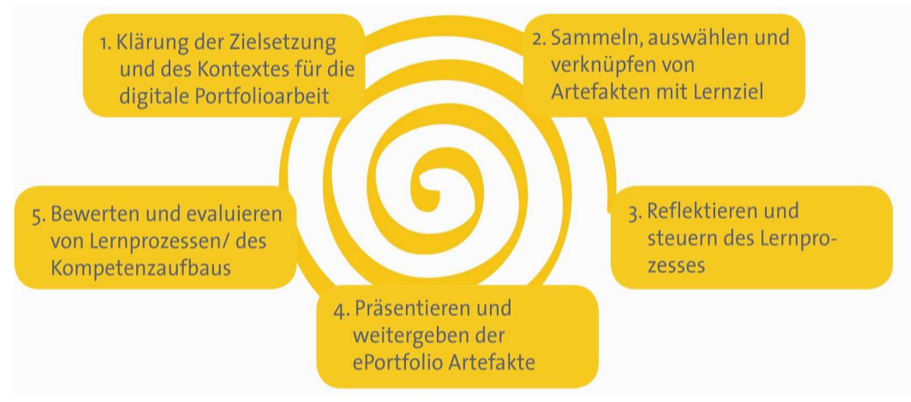
\includegraphics[width=0.7\linewidth]{e-portfolio-prozesse-schaffert}
		\caption{Prozesse der Portfolio-Arbeit (Schaffert et al. 2007, S. 79)\cite{schaffert_e-portfolio-einsatz_2007}}
		\label{fig:e-portfolio-prozesse-schaffert}
	\end{figure}
	\begin{figure}[h]
		\centering
		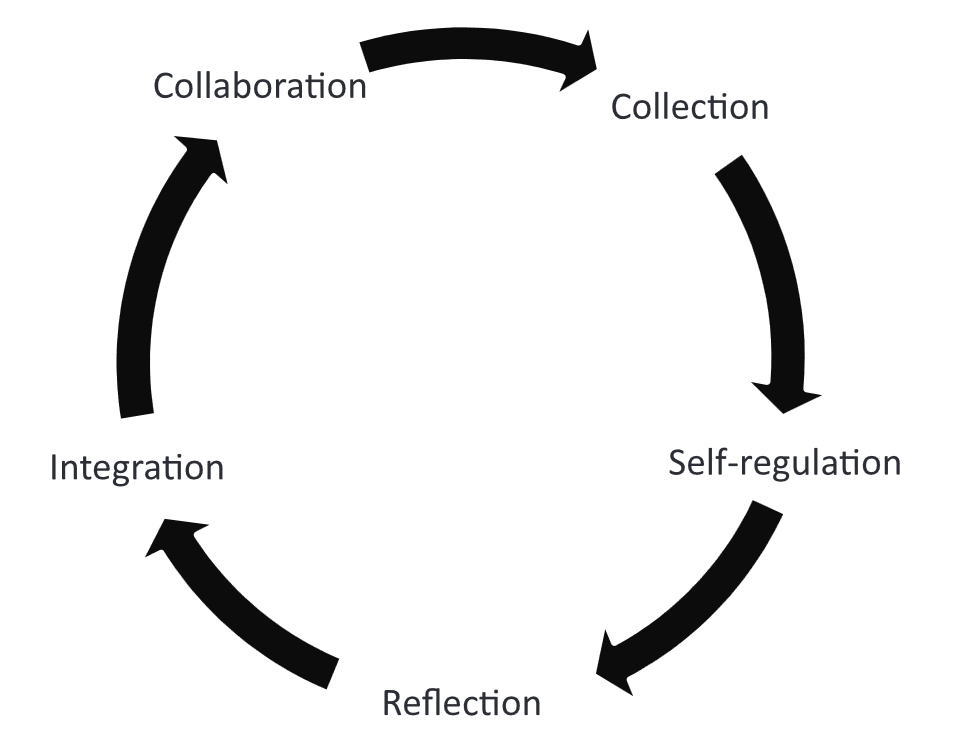
\includegraphics[width=0.5\linewidth]{cycle-of-documented-lifelong-learning-Jensen}
		\caption{cycle of documented lifelong learning (Jensen,Treuer 2014)\cite{jenson_defining_2014}}
		\label{fig:cycle-of-documented-lifelong-learning-jensen}
	\end{figure}
	\begin{figure}[h]
		\centering
		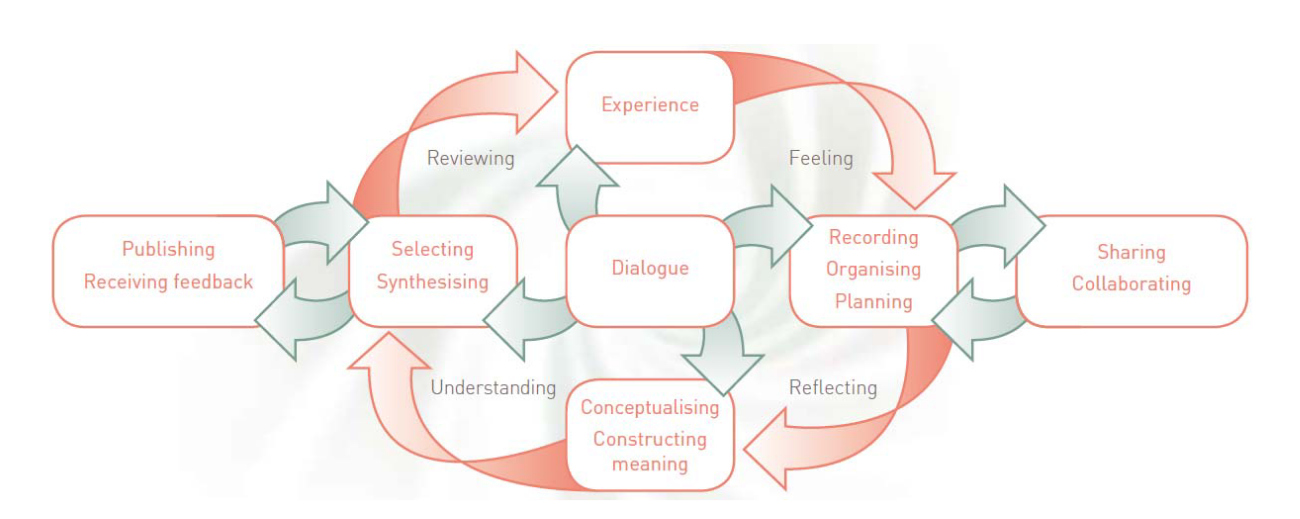
\includegraphics[width=0.8\linewidth]{model-of-e-portfolio-based-learning}
		\caption{A model of e-portfolio-based learning (JISC 2008, S. 9) \cite{jisc_effective_2008}}
		\label{fig:model-of-e-portfolio-based-learning}
	\end{figure}
	
	\pagebreak 
	
	\section*{Informationsmaterialien}
	
	Wiederhole dein Wissen über Latex oder nutze sonst im Notfall andere Editoren wie Word um PDF Dateien aus deinen Aufgaben und Artefakte, aber auch Scans, zu erstellen.\\
	Lese außerdem den Punkt 2.4. des \href{10.1016/j.sbspro.2010.03.463}{Artikels} \cite{alexiou_enhancing_2010}, und mache dir ein Bild zu selbst regulierendem Lernen.
	
	\bibliographystyle{alpha}
	\bibliography{../eportfolio_lib}
	
	\pagebreak
	
	\section*{Einleitung}
	Was bedeutet das Sammeln von Artefakten. Für diese Aufgabe kannst Du allein, oder mit einem Partner gemeinsam arbeiten. Der gemeinsame Aspekt an dieser Stelle liegt vor allem in dem Austausch von Fertigkeiten, wie Screenshots, PDF erstellen hochladen, usw.
	
	\section*{Aufgabenstellung}

	\begin{enumerate}
		\item Für dein Modul, sammle Aufgaben, die du gelöst und bearbeitet hast und verarbeite 2 Deiner besten Arbeiten in PDF-Dateien, bspw. dein Prüfungsvorleistungsprojekt. Versuche dabei in der Beschreibung diese Fragen mindestens zu beantworten:
		\begin{enumerate}
			\item Was war mein Anteil bei dieser Aufgabe?
			\item Was habe ich gelernt?
			\item Wie hat dies andere Menschen oder Dinge positiv beeinflusst?
		\end{enumerate}
		\item Für dein Studium, sammle aus mindestens 3 Modulen jeweils deine bestes Werk
		\begin{enumerate}
			\item Was war mein Anteil bei dieser Aufgabe?
			\item Was habe ich gelernt?
			\item Wie hat dies andere Menschen oder Dinge positiv beeinflusst?
		\end{enumerate}

	\end{enumerate}


\end{document}
